\chapter{Background}

\section{Reinforcement learning}

\paragraph{}
"The reinforcement learning problem is meant to be a straightforward framing of the problem of learning from interaction to
achieve a goal" \cite{sutton_barto_2018}. 
\begin{figure}[H]
    \centering
    \includegraphics[width=0.6\linewidth]{figures/agent-environment-interaction.png}
    \caption{Interaction of the agent with the environment during time step $t$. Figure taken from \cite{sutton_barto_2018}}
    \label{fig:agent-env-interaction}
\end{figure}

\paragraph{}
The reinforcement learning \textit{agent} continuously interacts with the \textit{environment}. This interaction can be modelled
as a sequence of time steps $t=0,1,2,3,...$\footnote{The interaction with the environment can also be modelled in continuous time,
however this is outside the scope of this project.}. At each step $t$, the environment is represented by its \textit{state} $S_t
\in \mathcal{S}$, where $\mathcal{S}$ is the set of all the possible states. Taking the \textit{state} as input, the agent outputs
an \textit{action} $a_t \in \mathcal{A}$, where $\mathcal{A}$ is the set of all the possible actions. In the next time step $t+1$,
the environment transitions to a new \textit{state}\footnote{Note that it is possible that $S_{t+1} = S_t$} $S_{t+1}$ and emits a
\textit{reward} $R_{t+1} \in \mathcal{R} \subset \R$, which the agent uses as feedback information to "learn" how to interact with
the environment. Each time step can then be represented by the $\langle S_t,A_t,R_{t+1},S_{t+1} \rangle$ tuple.

\paragraph{}
The agent implements a mapping from the possible states to the probabilities of choosing the different actions. This mapping is
called \textit{policy} and at time step $t$, it adopts symbol $\pi_t$. The probability of choosing action $A_t=a$ given the
current state $S_t=s$ is denoted by $\pi_t(a|s)$. The goal of reinforcement learning is to learn the optimal policy, which is the
policy that maximises the rewards, through repeated interaction with the environment. In general, we aim to maximise a function of
the rewards at all time steps rather than the immediate reward, so the optimal policy doesn't necessarily maximise immediate
rewards. The simplest case is to maximise  
\begin{equation}
    G_t =R_{t+1} + R_{t+2} + R_{t+3} + ... + R_T
\end{equation}
where $T$ is a final time step. This approach can be used when the agent-environment interaction has an end, in which case a
sequence of interactions from the initial time to time $T$ can be called an \textit{episode}. In other cases, the interactions can
continue indefinitely, thus this reward function is not feasible as $T=\infty$ and $G_t$ could be infinite. To fix this, we apply
a \textit{discount rate} $\gamma$, with  $|\gamma|<1$, to future rewards:
\begin{equation}
    G_t=R_{t+1} + \gamma R_{t+2} + \gamma^2 R_{t+3} + ... = 
    \sum_{k=0}^\infty \gamma^{k} R_{t+k+1}
\end{equation}
This allows $G_t$ to have a finite value in continuing tasks, which are those tasks that don't have finite time episodes.

\paragraph{}
In general, the dynamics of the environment could depend on the whole history of states, rewards and actions over an episode.
However, we aim to have an agent which can choose the optimal action at each time step based only on the current state. Thus the
knowledge of the current state and action should give the maximum possible amount of information about the dynamics of the
environment. This is true if knowledge of the history of states, rewards and actions in the previous time steps does not provide
any additional information about the dynamics of the environment than knowing the current state. States that follow this property
are said to follow the \textit{Markov property}. More formally, if the states follow this property
\begin{align}
    Pr\{R_{t+1}=r, S_{t+1}=s'|S_0,A_0,R_1,...,S_{t-1},A_{t-1},R_t,S_t,A_t\} \\
    = Pr\{R_{t+1}=r, S_{t+1}=s'|S_t,A_t\} \\
    = p(s',r|s,a)
\end{align}
This is the equation that governs Markov Decision Processes (MDPs) and hence a reinforcement learning task formulated with states
that follow the Markov property is an MDP. 
\begin{figure}[H]
    \centering
    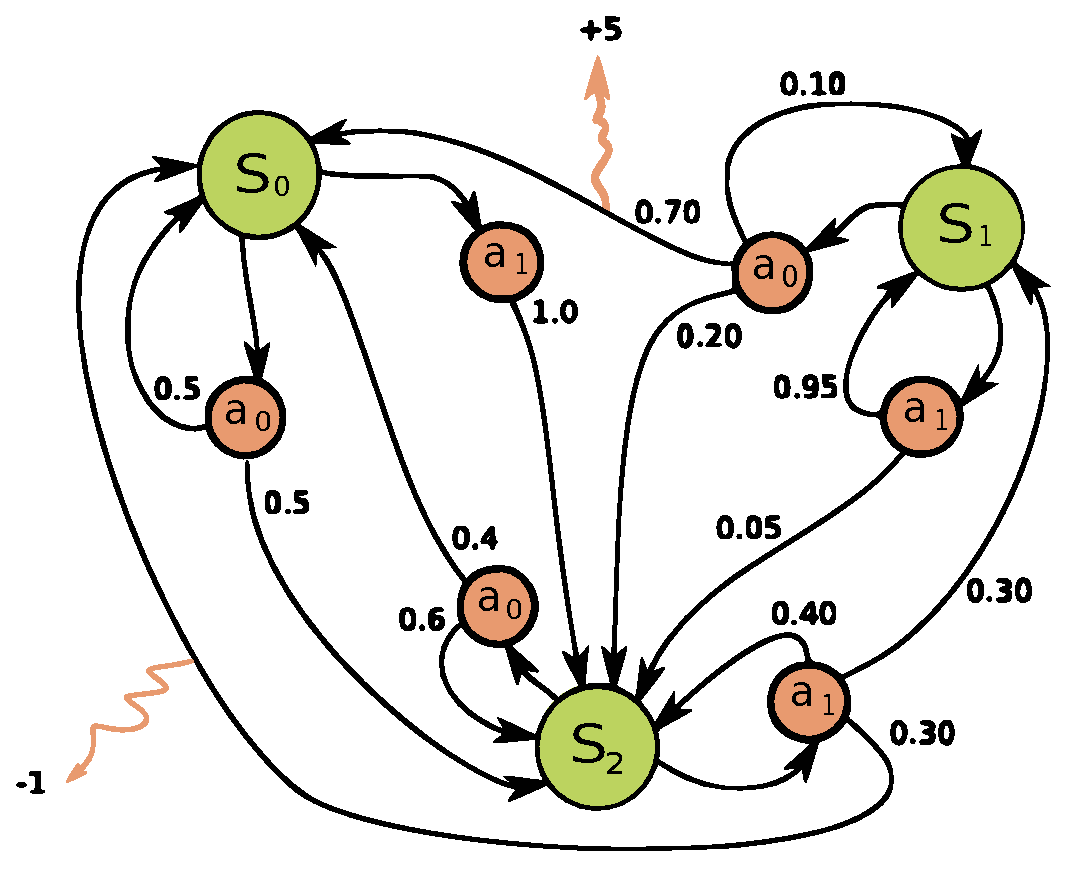
\includegraphics[width=0.5\linewidth]{figures/MDP.eps}
    \caption{Graph representation of a Markov Decision Process. Note the rewards (zigzag arrows) that are released in certain
    transitions. \cite{noauthor_markov_2021}}
    \label{fig:MDP}
\end{figure}

\paragraph{}
Most reinforcement learning algorithms involve the estimation of the \textit{value functions}, which are functions of states or
state-action pairs. A value function represents how good it is to be in a certain state or to perform a certain action in a
certain state, in terms of the expected return $G_t$ and given that we are following a certain policy. The action-value function
is defined as
\begin{equation}
    q_{\pi}(s,a)=\E_\pi[G_t|S_t=s,A_t=a]=\E_\pi\left[\sum_{k=0}^\infty \gamma^{k} R_{t+k+1}|S_t=s,A_t=a\right]
\end{equation}

Similarly, the state-value function is given by
\begin{align}
    v_{\pi}(s)=\E_\pi[G_t|S_t=s]\\
    =\E_\pi\left[\sum_{k=0}^\infty \gamma^{k} R_{t+k+1}|S_t=s\right]\\
    =\sum_a \pi(a|s) \E_\pi\left[\sum_{k=0}^\infty \gamma^{k} R_{t+k+1}|S_t=s,A_t=a\right]\\
    =\sum_a \pi(a|s) q_{\pi}(s,a)
\end{align}

It is useful to specify the value functions in recursive format, known as the Bellman equations. This gives:
\begin{align}
    v_{\pi}(s)=\E_\pi[G_t|S_t=s]\\
    =\E_\pi[R_{t+1}+\gamma G_{t+1}|S_t=s]\\
    =\sum_a \pi(a|s) \sum_{s',r}p(s',r|s,a)[r+v_\pi(s')]%, \,\,\, \forall s\in\mathcal{S}
\end{align}
and
\begin{align}
    q_{\pi}(s,a)=\E_\pi[G_t|S_t=s,A_t=a]\\
    =\E_\pi[R_{t+1}+\gamma G_{t+1}|S_t=s,A_t=a]\\
    =\sum_{s',r}p(s',r|s,a)[r+v_\pi(s')]%, \,\,\, \forall \in\mathcal{S}
\end{align}

\paragraph{}
For finite MDPs it can be proved that there always exists an \textit{optimal policy} that maximises the state-values of all states
the action-values of all state-action pairs, giving the optimal state-values $v_*(s)$ and $q_*(s,a)$:
\begin{align}
    v_*(s)=\max_\pi v_\pi(s), \,\,\, \forall s \in \mathcal{S} \\
    q_*(s,a)=\max_\pi q_\pi(s,a), \,\,\, \forall s \in \mathcal{S}, \,\,\, \forall a \in \mathcal{A}
\end{align}

\paragraph{}
Given full knowledge of the dynamics of the system\footnote{The probabilities of state-transitions and rewards given the current
state-action pair} and a fixed policy, we are able to evaluate the optimal state-values and action-values using methods based on
dynamic programming \cite{bellman_dynamic_1966}. One such method called \textit{iterative policy evaluation}, which adopts the
update step based on the Bellman equations given below, can be shown to converge to the state-values:

\begin{equation}
    v_{k+1}(s)=\sum_{a\in\mathcal{A}}\pi(a|s)\left[R(s,a)+\gamma\sum_{s'\in\mathcal{S}}P(s,s',a)v_k(s')\right]
\end{equation}

\textit{Policy iteration} is one possible method of evaluating the state values when the optimal policy is not given, which
alternates steps of policy evaluation and updates of the policy. The policy is updated so that in every state the greedy action,
meaning the one with the highest action-value, is always picked. This process of solving the MDP when given the model of the
environment is known as \textit{planning}. 

\paragraph{}
However, in many applications the model of the environment is unknown. Given a certain policy, it is possible in this case to
approximate the state and action values by sampling the interaction with the environment. Monte Carlo methods interact with the
environment by following the given policy and approximate each state-value using the returns obtained in each episode after the
first or each visit to the state. The update that occurs every time the state occurs for the first time in the episode  (or every
time, depending on the version of the algorithm) is
\begin{equation}
    V(S_t) \leftarrow V(S_t)+\alpha[G_t - V(S_t)]
\end{equation}
The disadvantage is that state-values cannot be updated until the end of an episode. Temporal Differences methods are another
class of methods that solve this problem. Instead of relying on returns ($G_t$), they approximate them as the sum of the reward
and the discounted state-value of the next visited state. The simplest TD algorithm's update step is given by
\begin{equation}
    V(S_t) \leftarrow V(S_t)+\alpha(R_{t+1} + \gamma V(S_{t+1})-V(S_t))
\end{equation}

\paragraph{}
There are many applications of reinforcement learning in which state-space and action-spaces are continuous. In that case, the MDP
is not finite as there is an infinite number of possible states and actions. This will not be discussed as it is outside of the
scope of this project, which only deals with discrete state and action spaces.

\section{Neural networks}
Should I give a bried intrdoction to neural networks

\section{Q-learning and Deep Q-learning}

SHOULD ADD A BIT OF INFORMATION ABOUT NEURAL NETWORKS

\paragraph{}
Many RL algorithms deal with the problem of solving an MDP without being given the optimal policy and the dynamics of the system.
Q-learning \cite{watkins_1989} is one of the most noteworthy among these. It is based on Temporal Differences learning as the
action-value updates follow a very similar formula. The basic value update in Q-learning is given by:
\begin{equation}
    Q(S_t, A_t) \leftarrow Q(S_t, A_t) + \alpha[R_{t+1}+\gamma \max_a Q(S_{t+1},a) - Q(S_t,a)]
\end{equation}
Differently from the previously described TD algorithm, this operates on action-values instead of state-values. In Q-learning, the
value update is done using the term $\max_a Q(S_{t+1},a)$, which is the action-value of the greedy-action in the next visited
state. This is not necessarily the action taken in the following step when visiting $S_{t+1}$, thus this an \textit{off-policy}
algorithm.

\paragraph{}
Differently from the Temporal Differences algorithms that aim at evaluating a fixed policy, Q-learning also deals with the control
problem of choosing the policy. Q-learning is normally programmed so that its current policy is based on its current action-value
estimates. An example is the $\epsilon$-greedy policy, in which at each time step, the greedy action is picked with probability
$1-\epsilon$ and a random action is picked with probability $\epsilon$.

\paragraph{}
This algorithm is only defined for discrete environments and it is proven to converge to the optimal action-values with a
probability of 1, as long as all the states and actions are visited multiple times \cite{watkins_q-learning_1992}. This
requirement might not be feasible when the number of states is very large and it is impossible when the number of states is
infinite such as when the MDP's state-space is continuous. Using a learned Q-function approximator instead of simply storing the
action-values in tabular form can solve this issue, as it is possible to learn a mapping function that generalises over the whole
state-space without having to visit all the possible states.

\paragraph{}
Deep Q-Learning (DQN) \cite{mnih_human-level_2015} implements the Q-function approximator using a deep neural network. This was
demonstrated to achieve state-of-the-art performance in learning to play Atari games directly from the pixel data \cite{dqn}. DQN
takes advantage of the ability of deep learning to learn from high-dimensional data representations to be able to directly feed
large state-spaces into the agent. Deep neural networks rely on the assumption that they are fed independent samples, however in
reinforcement learning the samples are correlated as they are generated by a temporal sequence. An \textit{experience replay} is
used to solve this. The transition samples are saved in memory and a random batch is selected to train the neural network at each
time-step, thus removing correlations due to temporal proximity of the samples. This also allows the update to be based on a
batch, rather than a single sample, which improves the sample efficiency\footnote{How efficiently the samples are used by the
algorithm to learn. A more sample efficient algorithm requires fewer interactions with the environment to learn an optimal
policy.}.

\paragraph{}
One issue of the Q-learning algorithm is that using the maximum action value of the next visited state in the update step results
in a positive bias in the estimation of the action values, which can lead to poor performance in some stochastic environments.
Double Q-learning \cite{wiskunde_doubleq-learning_nodate} deals with this problem by splitting the samples randomly between two
separate sets of action value estimates and by updating the values of each set of estimates using the values of the other, which
can be proven to remove the positive bias\footnote{It actually introduces a small negative bias, thus tending to underestimate the
action values.}. The same problem persists in deep Q-learning and a similar solution has been devised in Double Deep Q-Learning
\cite{van_hasselt_deep_2015}. Another version of DQN that achieved improved performance in typical benchmarks such as playing
Atari games is Dueling DQN \cite{wang_dueling_nodate}, which operates on the concept of expressing action values as a sum of state
values and advantages: $\mathcal{Q}_\pi(s,a)=\mathcal{V}_\pi(s)+\mathcal{A}_\pi(s,a)$.

\paragraph{}
While the original Q-learning algorithm can only be applied to systems with discrete state and action spaces, other algorithms
based on Q-learning have been proposed to deal with continuous state and action spaces, such as Wire Fitted Neural Network
Q-learning \cite{goos_q-learning_1999}.

\section{Problem of large state-spaces}

\paragraph{}
Very large systems correspond to MDPs with a very large number of states, which can be difficult to solve using reinforcement
learning algorithms. The number of possible state-transitions is the square of the number of states, thus the complexity of
controlling a system grows very quickly as the size of a system increases, and learning an optimal policy becomes very difficult
and often infeasible.

\paragraph{}
Various approaches have been used to solve this issue. One general approach is to learn representations of the states to improve
generalisation to unseen states or to decrease the dimensionality of the states by compression. DQN \cite{dqn} exploits the
ability of deep learning to learn from high-dimensional data and to generalise to solve this issue, though this is often not
sufficient. \cite{stateActionEmbeddings} jointly learns state and action embeddings to improve generalisation. In World Models
\cite{worldModels}, a compressed latent representation of the states is explicity learned by an autoencoder, which is then fed
into the reinforcement learning model instead of the original states. Other methods rely on state aggregation
\cite{stateAggregation}, in which states with similar state-transition probabilities and rewards are grouped to form a
higher-level state. This technique can also be applied to hierarchical reinforcement learning to define the states of the global
learner \cite{aggregationHierarchical}. 

\paragraph{}
Hierarchical reinforcement learning \cite{barto_recent_2003} is another approach that reduces the impact of large state spaces.
Hierarchical RL provides temporal abstraction by subdividing the main task into sub-tasks. For example, the task of commuting to
work can be subdivided into sub-tasks such as opening a door, turning right, walking to the tube station, etc. The agent is
composed of hierarchies of sub-agents in which each sub-agent is fed a compressed or reduced state space in input and outputs
high-level actions to its "children" sub-agents that perform the lower-level actions required to complete the received
higher-level action. Examples of hierarchical reinforcement learning algorithms are based on MAXQ value decomposition
\cite{dietterich_hierarchical_1999}, Options \cite{sutton_between_1999} and Hierarchies of Machines (HAM)
\cite{parr_reinforcement_nodate}. 

\paragraph{}
Model-based reinforcement learning \cite{moerland_model-based_2020} has been receiving increasing attention lately. This class of
algorithms is at the intersubsection of planning algorithms and model-free reinforcement learning as it approximates the model of the
environment during the learning process, which can be used to more efficiently learn from new samples. Dyna
\cite{sutton_dyna_1991} learns a model of the environment and uses it to simulate samples for Q-learning other than those obtained
by actual interaction with the environment. AlphaZero \cite{silver_mastering_2017}, which achieved state-of-the-art performance in
playing Chess, leverages full knowledge of the model\footnote{The model is given at the start rather than learnt.} to perform a
Monte-Carlo tree search for every step in the real-world environment. \cite{worldModels} trains an RNN model that predicts the
following state at each-time step. Though this class of algorithms does not explicitly tackle the problem of large state-spaces,
the improvements in sample efficiency can still solve the issue by allowing to train a model with fewer interactions with the
environment. 
